\documentclass{article}
\usepackage[utf8]{inputenc}
\usepackage[french]{babel}
\usepackage[T1]{fontenc}
\usepackage{algorithm}
\usepackage{graphicx}
\usepackage{float}
\usepackage{listings}
\usepackage{xcolor}

\title{}
\author{}
\date{}


\setlength{\parindent}{0cm}
\setlength{\parskip}{1ex plus 0.5ex minus 0.2ex}
\newcommand{\hsp}{\hspace{20pt}}
\newcommand{\HRule}{\rule{\linewidth}{0.5mm}}


\title{}
\author{}
\date{}

\makeatletter
\def\BState{\State\hskip-\ALG@thistlm}
\makeatother

\lstset{basicstyle = \ttfamily,columns=fullflexible}


\begin{document}

\begin{titlepage}
  \begin{sffamily}
  \begin{center}

    % Upper part of the page. The '~' is needed because \\
    % only works if a paragraph has started.

    \textsc{\LARGE Polytech Sorbonne}\\[2cm]

    \textsc{\Large EPU-N7-IOB}\\[1.5cm]

    % Title
    \HRule \\[0.4cm]
    { \huge \bfseries Projet final: Space Invader v2\\[0.4cm] }

    \HRule \\[2cm]
    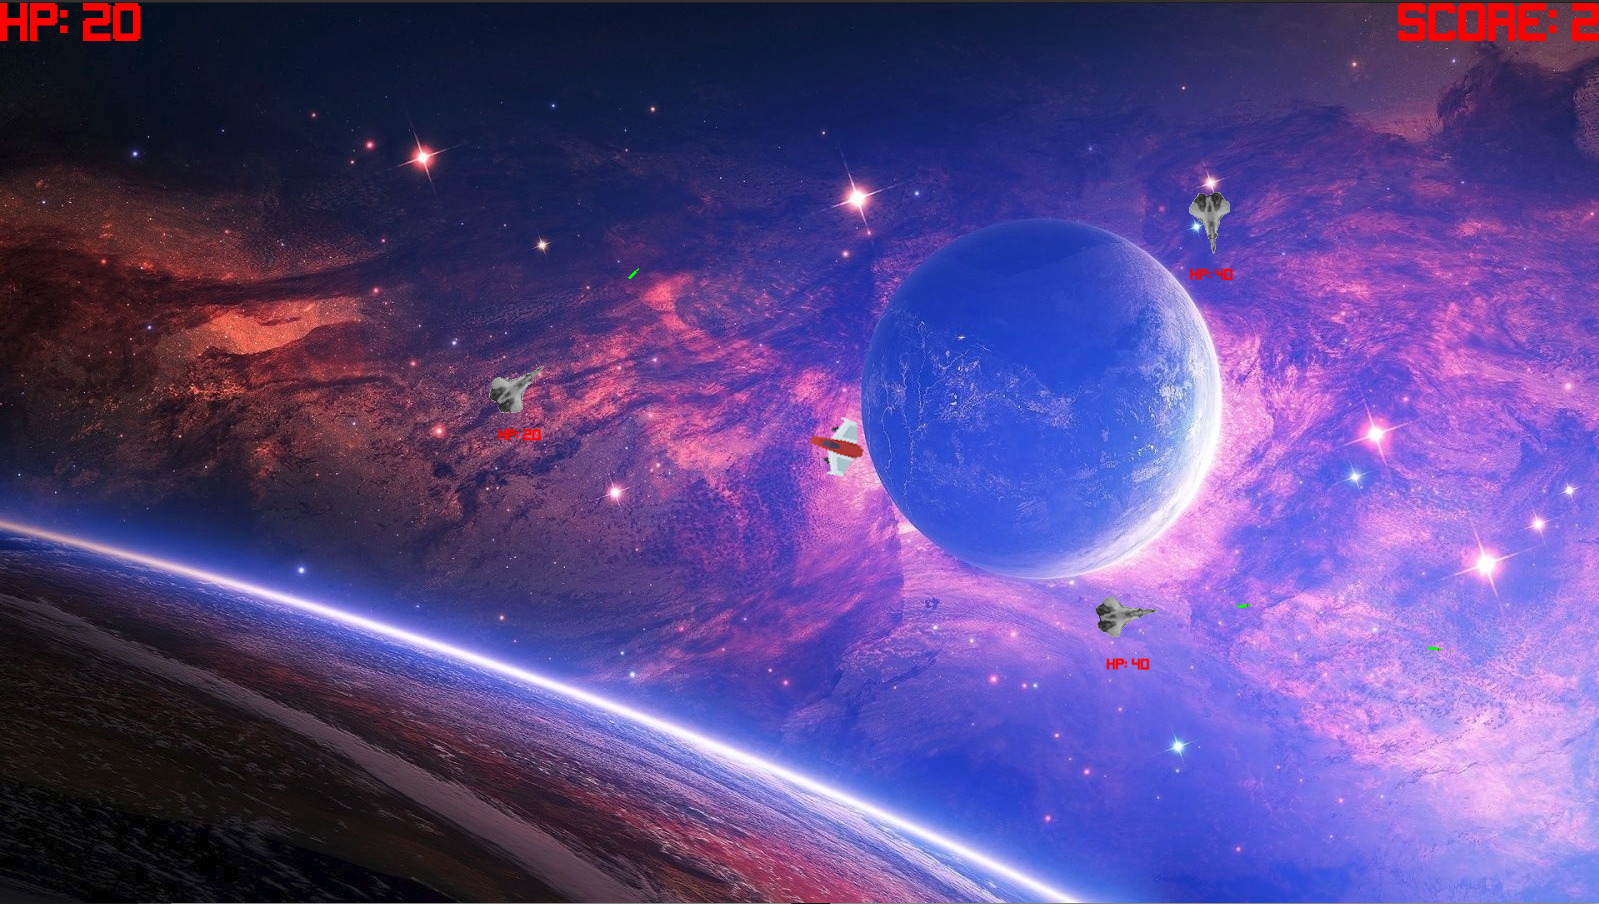
\includegraphics[width=1\textwidth]{assets/img/illustration.png}
    \\[2cm]

    \vfill
    \begin{minipage}{0.4\textwidth}
      \begin{center} \large
        Arthur Guillec\\
      \end{center}
    \end{minipage}
    \vfill

  \end{center}
  \end{sffamily}
\end{titlepage}


\section{Introduction}

Ce rapport est joint aux sources du projet final du cours \textbf{Language objet – C++-UML} dispensé en 4e année de MAIN par.

\section{Le jeu}

L'objectif est similaire à celui du jeu \textbf{Space Invaders}. Le joueur est aux commandes d'un vaisseau spatial et doit se défendre face à une horde d'ennemis déterminés.

Il est possible de se déplacer dans toutes les directions du plan 2D. A chaque fois qu'un vaisseau ennemi est détruit, le score du joueur s'incrémente de un. L'objectif est d'avoir le plus grand score à la fin de la partie, i.e lorsque le vaisseau du joueur n'a plus de vie.

\subsection{Dépendances}

La partie audio et graphique du programme nécessite la bibliothèque \textbf{SFML} (Simple and Fast Multimedia Library). Elle s'installe facilement sur Debian et ses dérivés via la commande:

\begin{lstlisting}[language=bash]
$ sudo apt-get install libsfml-dev
\end{lstlisting}

\subsection{Compilation}

Les sources du programme peuvent être récupérés depuis le dépôt \textbf{GIT} via la commande

\begin{lstlisting}[language=bash]
$ git clone https://github.com/3700240/guillec-projet-cpp
\end{lstlisting}

Un Makefile contenant une règle \textbf{all} et \textbf{clean} est fournit. Une fois la bibliothèque \textbf{SFML} installée, il ne reste donc plus qu'à exécuter la commande

\begin{lstlisting}[language=bash]
$ make
\end{lstlisting}

depuis le répertoire guillec-projet-cpp. puis

\begin{lstlisting}[language=bash]
$ ./game.bin
\end{lstlisting}

pour lancer une partie. Bon jeu!

\section{Les classes}


\subsection{Entity}

\subsection{ResourceManager}

\subsection{GameInstance}

\section{Conclusion}

\end{document}